\chapter{\textsf{\acronym}}
\section*{Description}
\emph{NUXIS} is a centralized tool that allows the management of available resources on a network. It consists of a Linux distribution pre-installed and configured, which allows you to manage servers' resources.

The \acronym is divided into two functional blocks:

\begin{itemize}
	\item \emph{Central Management} (CM)
    \item \emph{Virtualization Agent} (VA)
\end{itemize}

\begin{figure}[H]
	\begin{center}
	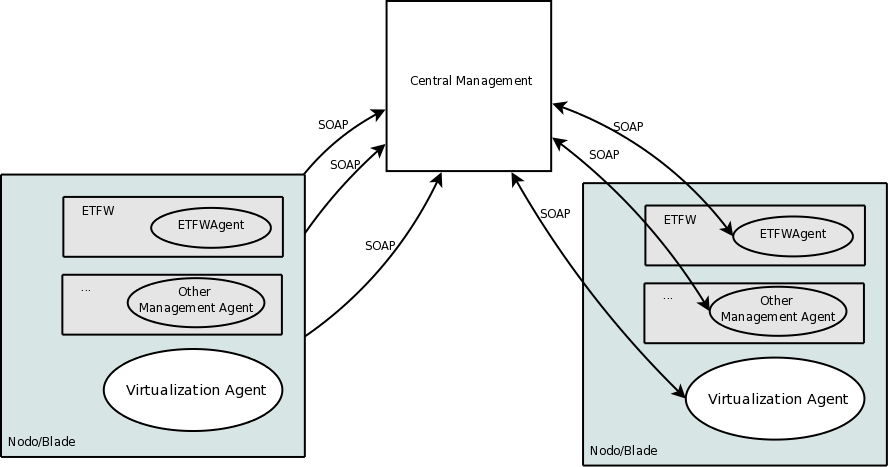
\includegraphics[scale=0.35]{screenshots/etva_blocos.png}
	\caption{\acronym architecture}
	\label{fig:etva_blocos}
	\end{center}
\end{figure}

The CM (Central Management) is the block responsible for managing the entire infrastructure.
The \emph{Virtualization Agents} are responsible for processing the requests between the virtualization server (\emph{node}) and CM.

Within a virtualization server there may be virtual machines with \emph{Management Agents}. These type agent enables the managing of existing services/applications on the virtual machine (see Figure \ref{fig:etva_blocos}).

In the \acronym, there are several virtualization servers (nodes) that communicate with the CM. The initial network configuration is performed, using VLANs through the \emph{One time setup wizard} as shown in Figure \ref{fig:first_time_wizard}.

\begin{figure}[H]
    \begin{center}
	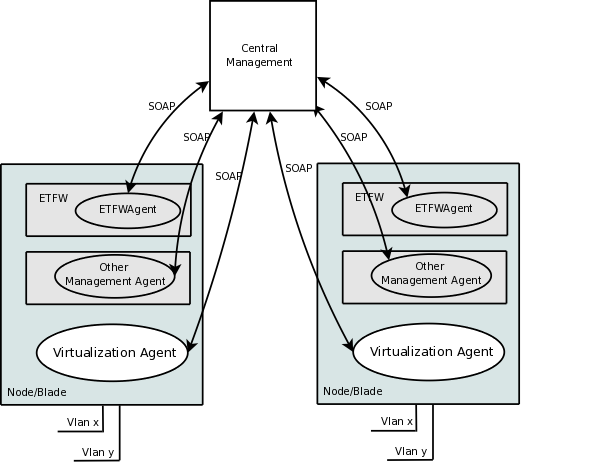
\includegraphics[scale=0.6]{screenshots/etva_enterprise.png}
	\caption{\acronym model}
	\label{fig:etva_enterprise}
	\end{center}
\end{figure}

This user's manual describes the configuration management tool (CM - \emph{Central Management}). 

\pagebreak
%\chapter{\textsf{Instalação}}
%\label{chp:installation}
%
%\pagebreak
